\documentclass{standalone}
\usepackage{tikz}
\usetikzlibrary{patterns, positioning}

\begin{document}
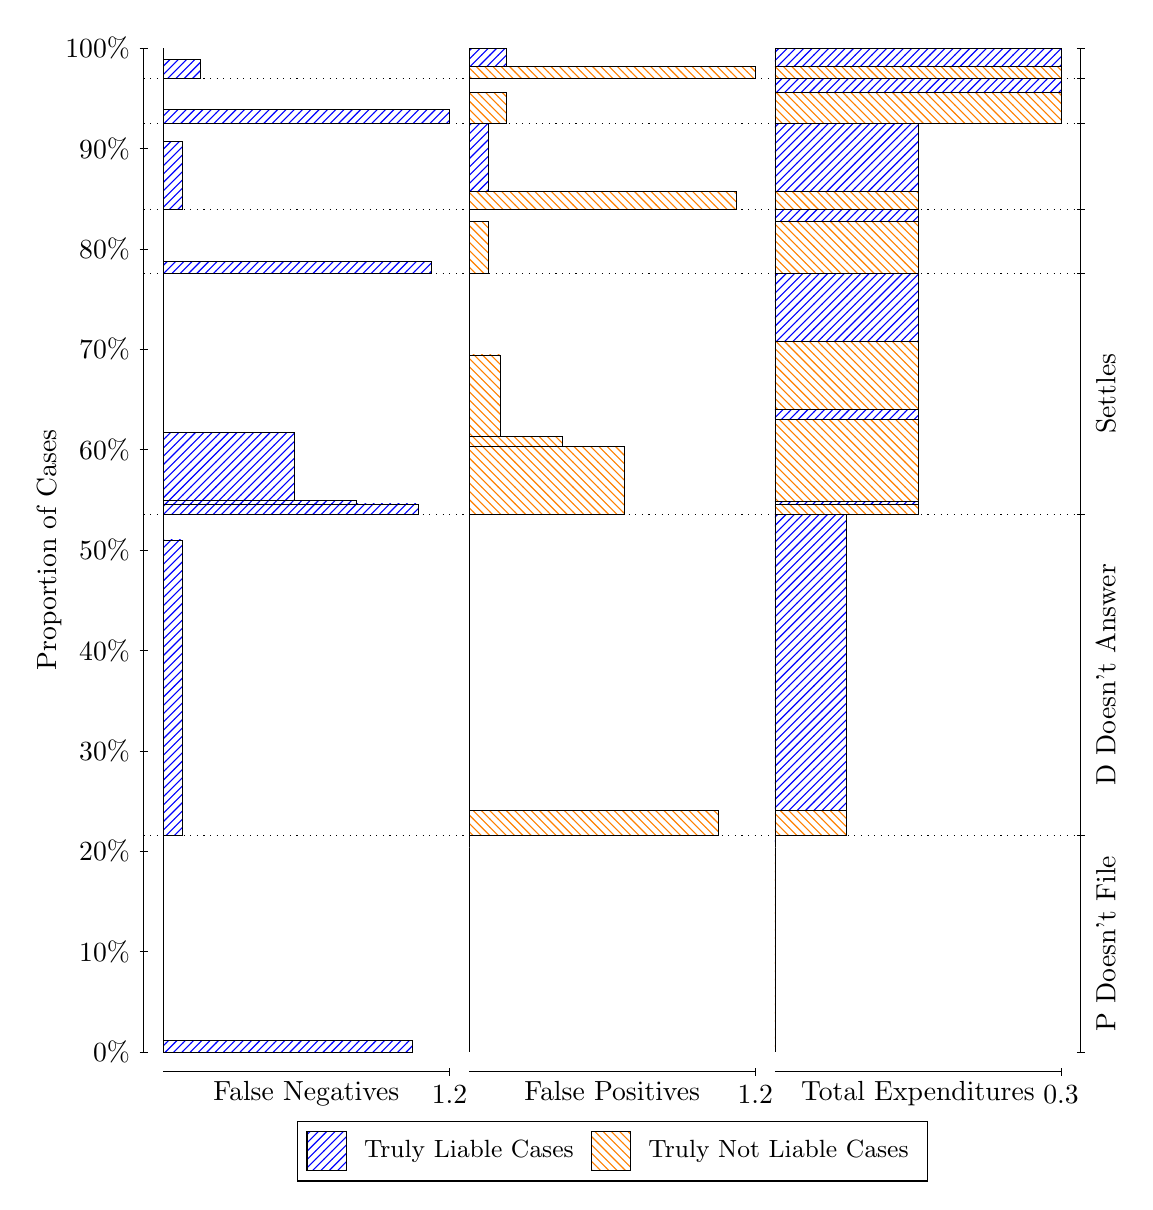
\begin{tikzpicture}
\draw[black, very thin] (1.5,1.75) -- (1.5,14.5);
\node[rotate=90, anchor=center] at (0.3, 8.125) {Proportion of Cases};
\draw[black, very thin] (1.45,1.75) -- (1.55,1.75);
\node[anchor=east] at (1.45, 1.75) {0\%};
\draw[black, very thin] (1.45,3.025) -- (1.55,3.025);
\node[anchor=east] at (1.45, 3.025) {10\%};
\draw[black, very thin] (1.45,4.3) -- (1.55,4.3);
\node[anchor=east] at (1.45, 4.3) {20\%};
\draw[black, very thin] (1.45,5.575) -- (1.55,5.575);
\node[anchor=east] at (1.45, 5.575) {30\%};
\draw[black, very thin] (1.45,6.85) -- (1.55,6.85);
\node[anchor=east] at (1.45, 6.85) {40\%};
\draw[black, very thin] (1.45,8.125) -- (1.55,8.125);
\node[anchor=east] at (1.45, 8.125) {50\%};
\draw[black, very thin] (1.45,9.4) -- (1.55,9.4);
\node[anchor=east] at (1.45, 9.4) {60\%};
\draw[black, very thin] (1.45,10.675) -- (1.55,10.675);
\node[anchor=east] at (1.45, 10.675) {70\%};
\draw[black, very thin] (1.45,11.95) -- (1.55,11.95);
\node[anchor=east] at (1.45, 11.95) {80\%};
\draw[black, very thin] (1.45,13.225) -- (1.55,13.225);
\node[anchor=east] at (1.45, 13.225) {90\%};
\draw[black, very thin] (1.45,14.5) -- (1.55,14.5);
\node[anchor=east] at (1.45, 14.5) {100\%};

\draw[black, very thin] (13.4,1.75) -- (13.4,14.5);
\draw[black, very thin] (13.35,1.75) -- (13.45,1.75);
\node[anchor=west] at (13.35, 1.75) {};
\draw[black, very thin] (13.35,4.4974) -- (13.45,4.4974);
\node[anchor=west] at (13.35, 4.4974) {};
\draw[black, very thin] (13.35,8.5794) -- (13.45,8.5794);
\node[anchor=west] at (13.35, 8.5794) {};
\draw[black, very thin] (13.35,11.638) -- (13.45,11.638);
\node[anchor=west] at (13.35, 11.638) {};
\draw[black, very thin] (13.35,12.452) -- (13.45,12.452);
\node[anchor=west] at (13.35, 12.452) {};
\draw[black, very thin] (13.35,13.541) -- (13.45,13.541);
\node[anchor=west] at (13.35, 13.541) {};
\draw[black, very thin] (13.35,14.114) -- (13.45,14.114);
\node[anchor=west] at (13.35, 14.114) {};
\draw[black, very thin] (13.35,14.5) -- (13.45,14.5);
\node[anchor=west] at (13.35, 14.5) {};

\draw[black, very thin, pattern color=blue, pattern=north east lines] (1.75,1.75) rectangle (4.9094,1.9014);
\draw[black, very thin, pattern color=orange, pattern=north west lines] (1.75,1.9014) rectangle (1.75,4.4974);
\draw[black, very thin, pattern color=blue, pattern=north east lines] (1.75,4.4974) rectangle (1.987,8.254);
\draw[black, very thin, pattern color=orange, pattern=north west lines] (1.75,8.254) rectangle (1.75,8.5794);
\draw[black, very thin, pattern color=blue, pattern=north east lines] (1.75,8.5794) rectangle (4.9884,8.7098);
\draw[black, very thin, pattern color=blue, pattern=north east lines] (1.75,8.7098) rectangle (4.1986,8.7529);
\draw[black, very thin, pattern color=blue, pattern=north east lines] (1.75,8.7529) rectangle (3.4087,9.6154);
\draw[black, very thin, pattern color=orange, pattern=north west lines] (1.75,9.6154) rectangle (1.75,11.638);
\draw[black, very thin, pattern color=blue, pattern=north east lines] (1.75,11.638) rectangle (5.1464,11.791);
\draw[black, very thin, pattern color=orange, pattern=north west lines] (1.75,11.791) rectangle (1.75,12.452);
\draw[black, very thin, pattern color=blue, pattern=north east lines] (1.75,12.452) rectangle (1.987,13.312);
\draw[black, very thin, pattern color=orange, pattern=north west lines] (1.75,13.312) rectangle (1.75,13.541);
\draw[black, very thin, pattern color=blue, pattern=north east lines] (1.75,13.541) rectangle (5.3833,13.722);
\draw[black, very thin, pattern color=orange, pattern=north west lines] (1.75,13.722) rectangle (1.75,14.114);
\draw[black, very thin, pattern color=blue, pattern=north east lines] (1.75,14.114) rectangle (2.2239,14.351);
\draw[black, very thin, pattern color=orange, pattern=north west lines] (1.75,14.351) rectangle (1.75,14.5);
\draw[black, very thin, pattern color=orange, pattern=north west lines] (5.6333,1.75) rectangle (5.6333,4.346);
\draw[black, very thin, pattern color=blue, pattern=north east lines] (5.6333,4.346) rectangle (5.6333,4.4974);
\draw[black, very thin, pattern color=orange, pattern=north west lines] (5.6333,4.4974) rectangle (8.7928,4.8228);
\draw[black, very thin, pattern color=blue, pattern=north east lines] (5.6333,4.8228) rectangle (5.6333,8.5794);
\draw[black, very thin, pattern color=orange, pattern=north west lines] (5.6333,8.5794) rectangle (7.608,9.4419);
\draw[black, very thin, pattern color=orange, pattern=north west lines] (5.6333,9.4419) rectangle (6.8181,9.5632);
\draw[black, very thin, pattern color=orange, pattern=north west lines] (5.6333,9.5632) rectangle (6.0283,10.602);
\draw[black, very thin, pattern color=blue, pattern=north east lines] (5.6333,10.602) rectangle (5.6333,11.638);
\draw[black, very thin, pattern color=orange, pattern=north west lines] (5.6333,11.638) rectangle (5.8703,12.299);
\draw[black, very thin, pattern color=blue, pattern=north east lines] (5.6333,12.299) rectangle (5.6333,12.452);
\draw[black, very thin, pattern color=orange, pattern=north west lines] (5.6333,12.452) rectangle (9.0297,12.681);
\draw[black, very thin, pattern color=blue, pattern=north east lines] (5.6333,12.681) rectangle (5.8703,13.541);
\draw[black, very thin, pattern color=orange, pattern=north west lines] (5.6333,13.541) rectangle (6.1072,13.933);
\draw[black, very thin, pattern color=blue, pattern=north east lines] (5.6333,13.933) rectangle (5.6333,14.114);
\draw[black, very thin, pattern color=orange, pattern=north west lines] (5.6333,14.114) rectangle (9.2667,14.263);
\draw[black, very thin, pattern color=blue, pattern=north east lines] (5.6333,14.263) rectangle (6.1072,14.5);
\draw[black, very thin, pattern color=orange, pattern=north west lines] (9.5167,1.75) rectangle (9.5167,4.346);
\draw[black, very thin, pattern color=blue, pattern=north east lines] (9.5167,4.346) rectangle (9.5167,4.4974);
\draw[black, very thin, pattern color=orange, pattern=north west lines] (9.5167,4.4974) rectangle (10.425,4.8228);
\draw[black, very thin, pattern color=blue, pattern=north east lines] (9.5167,4.8228) rectangle (10.425,8.5794);
\draw[black, very thin, pattern color=orange, pattern=north west lines] (9.5167,8.5794) rectangle (11.333,8.7006);
\draw[black, very thin, pattern color=blue, pattern=north east lines] (9.5167,8.7006) rectangle (11.333,8.7438);
\draw[black, very thin, pattern color=orange, pattern=north west lines] (9.5167,8.7438) rectangle (11.333,9.7826);
\draw[black, very thin, pattern color=blue, pattern=north east lines] (9.5167,9.7826) rectangle (11.333,9.9131);
\draw[black, very thin, pattern color=orange, pattern=north west lines] (9.5167,9.9131) rectangle (11.333,10.776);
\draw[black, very thin, pattern color=blue, pattern=north east lines] (9.5167,10.776) rectangle (11.333,11.638);
\draw[black, very thin, pattern color=orange, pattern=north west lines] (9.5167,11.638) rectangle (11.333,12.299);
\draw[black, very thin, pattern color=blue, pattern=north east lines] (9.5167,12.299) rectangle (11.333,12.452);
\draw[black, very thin, pattern color=orange, pattern=north west lines] (9.5167,12.452) rectangle (11.333,12.681);
\draw[black, very thin, pattern color=blue, pattern=north east lines] (9.5167,12.681) rectangle (11.333,13.541);
\draw[black, very thin, pattern color=orange, pattern=north west lines] (9.5167,13.541) rectangle (13.15,13.933);
\draw[black, very thin, pattern color=blue, pattern=north east lines] (9.5167,13.933) rectangle (13.15,14.114);
\draw[black, very thin, pattern color=orange, pattern=north west lines] (9.5167,14.114) rectangle (13.15,14.263);
\draw[black, very thin, pattern color=blue, pattern=north east lines] (9.5167,14.263) rectangle (13.15,14.5);
\draw[black, dotted] (1.5,4.4974) -- (13.4,4.4974);
\draw[black, dotted] (1.5,8.5794) -- (13.4,8.5794);
\draw[black, dotted] (1.5,11.638) -- (13.4,11.638);
\draw[black, dotted] (1.5,12.452) -- (13.4,12.452);
\draw[black, dotted] (1.5,13.541) -- (13.4,13.541);
\draw[black, dotted] (1.5,14.114) -- (13.4,14.114);
\draw[black, very thin] (1.75,1.5) -- (5.3833,1.5);
\node[anchor=north] at (3.5667, 1.5) {False Negatives};
\draw[black, very thin] (5.3833,1.45) -- (5.3833,1.55);
\node[anchor=north] at (5.3833, 1.45) {1.2};

\draw[black, very thin] (5.6333,1.5) -- (9.2667,1.5);
\node[anchor=north] at (7.45, 1.5) {False Positives};
\draw[black, very thin] (9.2667,1.45) -- (9.2667,1.55);
\node[anchor=north] at (9.2667, 1.45) {1.2};

\draw[black, very thin] (9.5167,1.5) -- (13.15,1.5);
\node[anchor=north] at (11.333, 1.5) {Total Expenditures};
\draw[black, very thin] (13.15,1.45) -- (13.15,1.55);
\node[anchor=north] at (13.15, 1.45) {0.3};

\node[black, centered, rotate=90] at (13.72, 3.1237) {P Doesn't File};
\node[black, centered, rotate=90] at (13.72, 6.5384) {D Doesn't Answer};
\node[black, centered, rotate=90] at (13.72, 10.109) {Settles};





\draw (7.449999999999999,1.5) node[draw=none] (baseCoordinate) {};
\begin{scope}[align=center]
        \matrix[scale=0.5, draw=black, below=0.5cm of baseCoordinate, nodes={draw}, column sep=0.1cm]{
            \node[rectangle, draw, minimum width=0.5cm, minimum height=0.5cm, pattern=north east lines, pattern color=blue] {}; &
            \node[draw=none, font=\small] (B) {Truly Liable Cases}; &
            \node[rectangle, draw, minimum width=0.5cm, minimum height=0.5cm, pattern=north west lines, pattern color=orange] {}; &
            \node[draw=none, font=\small] (B) {Truly Not Liable Cases}; \\
            };
\end{scope}

\end{tikzpicture}
\end{document}